% !TEX root = BIGALL-Master.tex
\section{Messungen und Auswertung}

\subsection{Synthese Kupfersulfidnanopartikel}
	Bei dieser Synthese war das Ziel Kupfersulfid aus dem Single-Source-Precursor \ch{Cu[DDTC]2} als Nanopartikel herzustellen. 
	Die Partikel wurden per UV-vis-NIR-Spektroskopie und mit TEM untersucht.
	Das Absorptionsspektrum zeigt ein Maximum bei $\lambda_{max}$=\SI{330}{\nano\meter}, mit einer kleinen Schulter bei \SI{360}{\nano\meter}.
	Die TEM Bilder zeigen, dass die Nanopartikel eine hexagonale Form besitzen und etwa \SI{350}{\nano\meter} als Durchmesser besitzen.
	Die Partikel sind so erstmal viel größer, als später die Partikel und Gele um die sich die Schale bilden soll.
	Dies sollte allerdings kein Problem darstellen, da sobald diese Synthese in Anwesenheit von anderen Partikel stattfindet diese das Nukleationsverhalten beeinflussen können.
	
	
	\begin{figure}[H]
		\centering
		\includegraphics[width=0.6\textwidth]{Bilder/UV-CuS} 	
		\caption{Absorptionsspektrum der CuS-Nanopartikel in Toluol, gemessen in einer Ulbrichtkugel.}
		\label{fig:UV-CuS}
	\end{figure}
	
	\begin{figure}[H]
		\centering
		\includegraphics[width=0.6\textwidth]{Bilder/TEM-CuS} 	
		\caption{TEM-Bild der CuS-Nanopartikel.}
		\label{fig:TEM-CuS}
	\end{figure}
	
\subsection{Synthese Goldnanopartikel}
	Bei dieser Synthese war es das Ziel möglichst monodisperse Goldnanopartikel herzustellen.
	Die Partikel wurden per UV-vis-Spektroskopie und mit TEM untersucht.
	Das UV-vis zeigt ein für Gold typisches, durch LOPR bedingte, Absorptionsmaximum von $\lambda_{Gold}$=\SI{519}{\nano\meter}, wie in \cref{fig:UV-AuNP} dargestellt.
	Aus den TEM-Bildern geht hervor, dass die Partikel eine mittlere Größe von etwa \SI{7,6}{\nano\meter} mit einer Abweichung von etwa \SI{0,6}{\nano\meter}, wie \cref{fig:TEM-Au-Hex-2} zeigt.	
	Die Partikel zeigten also eine zufriedenstellende Größenverteilung und können somit für weitere Experimente verwendet werden.
	
	\begin{figure}[H]
		\centering
		\includegraphics[width=0.6\textwidth]{Bilder/Gold-NP-Organisch} 	
		\caption{Absorptionsspektrum der Goldnanopartikel in Hexan gemessen.}
		\label{fig:UV-AuNP}
	\end{figure}
	
	\begin{figure}[htbp]
		\centering
		\subfloat[\label{fig:TEM-Au-Hex}]{%
			\includegraphics[width=0.45\linewidth]{Bilder/TEM-Au-Hex}}
		\subfloat[\label{fig:Size-Gold-NP}]{%
			\includegraphics[width=0.45\linewidth]{Bilder/Size-Gold-NP-Organisch}}
		\caption{\emph{(a)}: TEM-Aufnahme der Gold-NP und \emph{(b)}: Größenverteilung}
		\label{fig:TEM-Au-Hex-2}
	\end{figure}

	

	
	
\subsection{Synthese von CuS mit \ch{Cu[DDTC]2} und \ch{CuCl2}}

	Bei der Synthese von \ch{Cu[DDTC]2} und \ch{CuCl2} zeigt sich deutlich der Einfluss des \ch{CuCl2}. 
	Während bei reinem \ch{Cu[DDTC]2} die Partikel auf eine Größe von über \SI{300}{\nano\meter} wachsen und es dementsprechend wenig Partikel gibt, zeigen die TEM-Aufnahmen, die in \cref{fig:TEM-CuCl} gezeigt sind, hier dass es zu vielen kleinen Partikeln in der Größe von Quantenpunkten kommt.
	
	\begin{figure}[H]
		\centering
		\subfloat[\label{fig:CuCl-1}]{%
		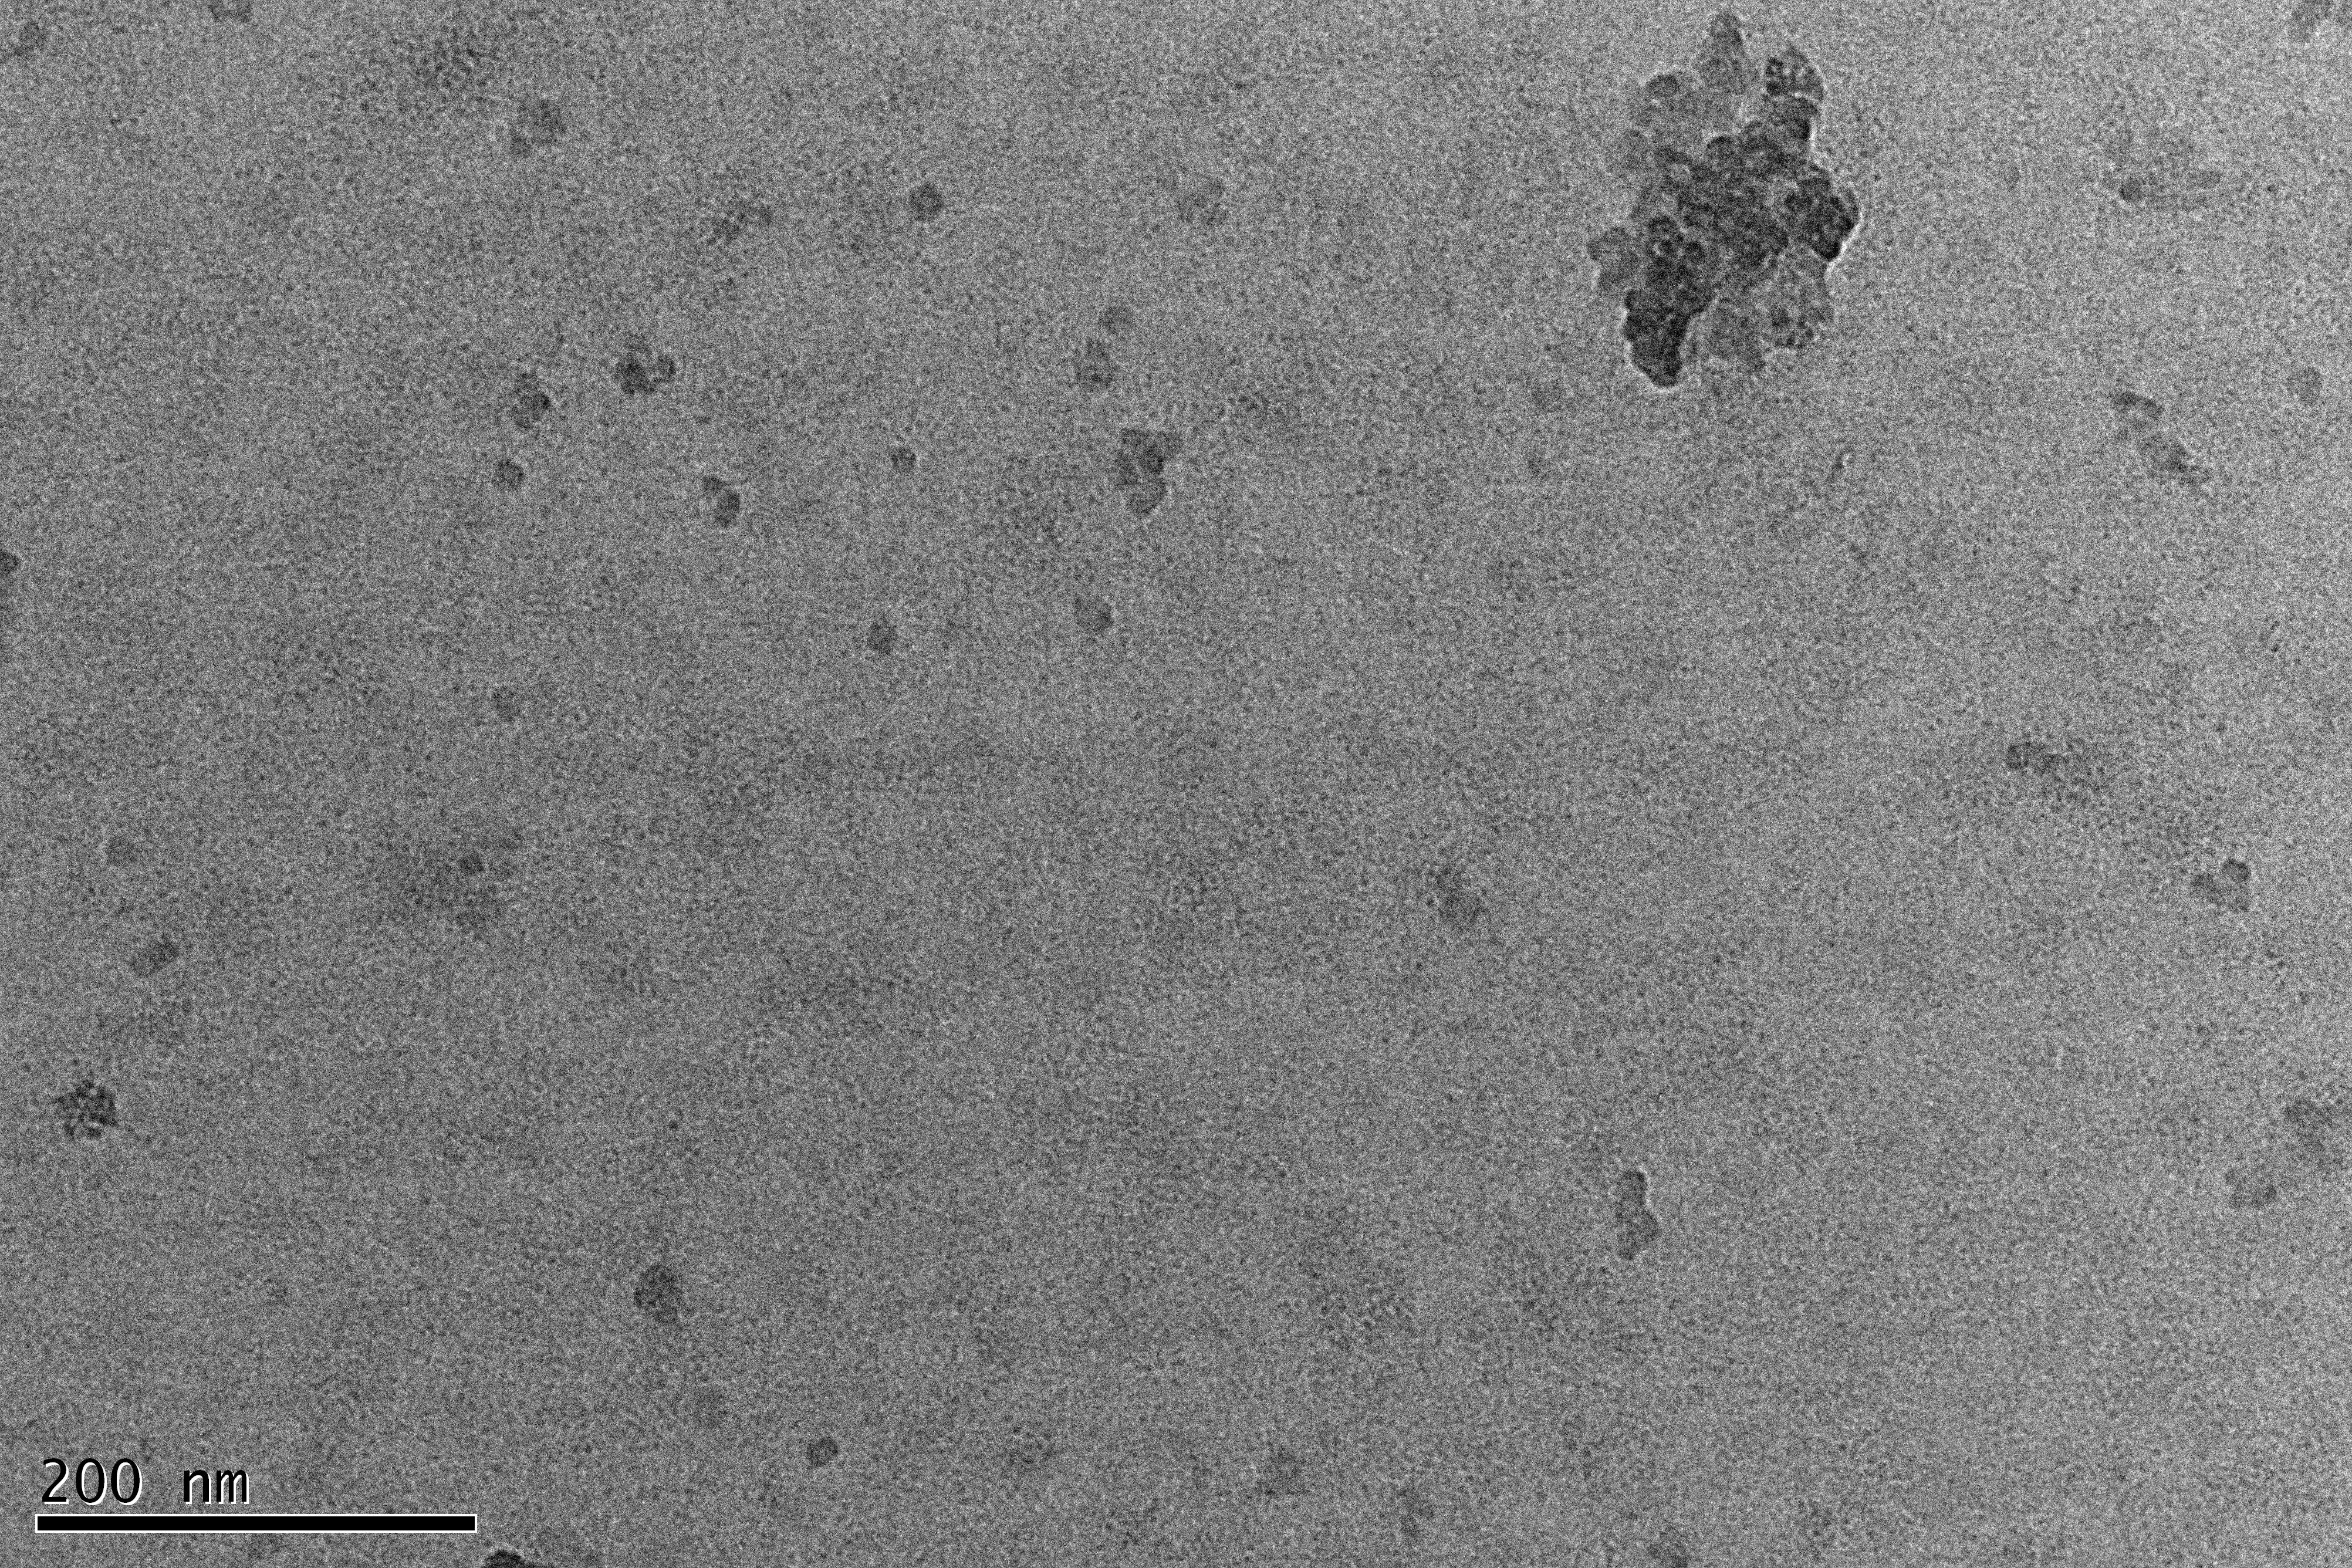
\includegraphics[width=0.45\linewidth]{Bilder/CuCl-1}}
		\subfloat[\label{fig:CuCl-2}]{%
		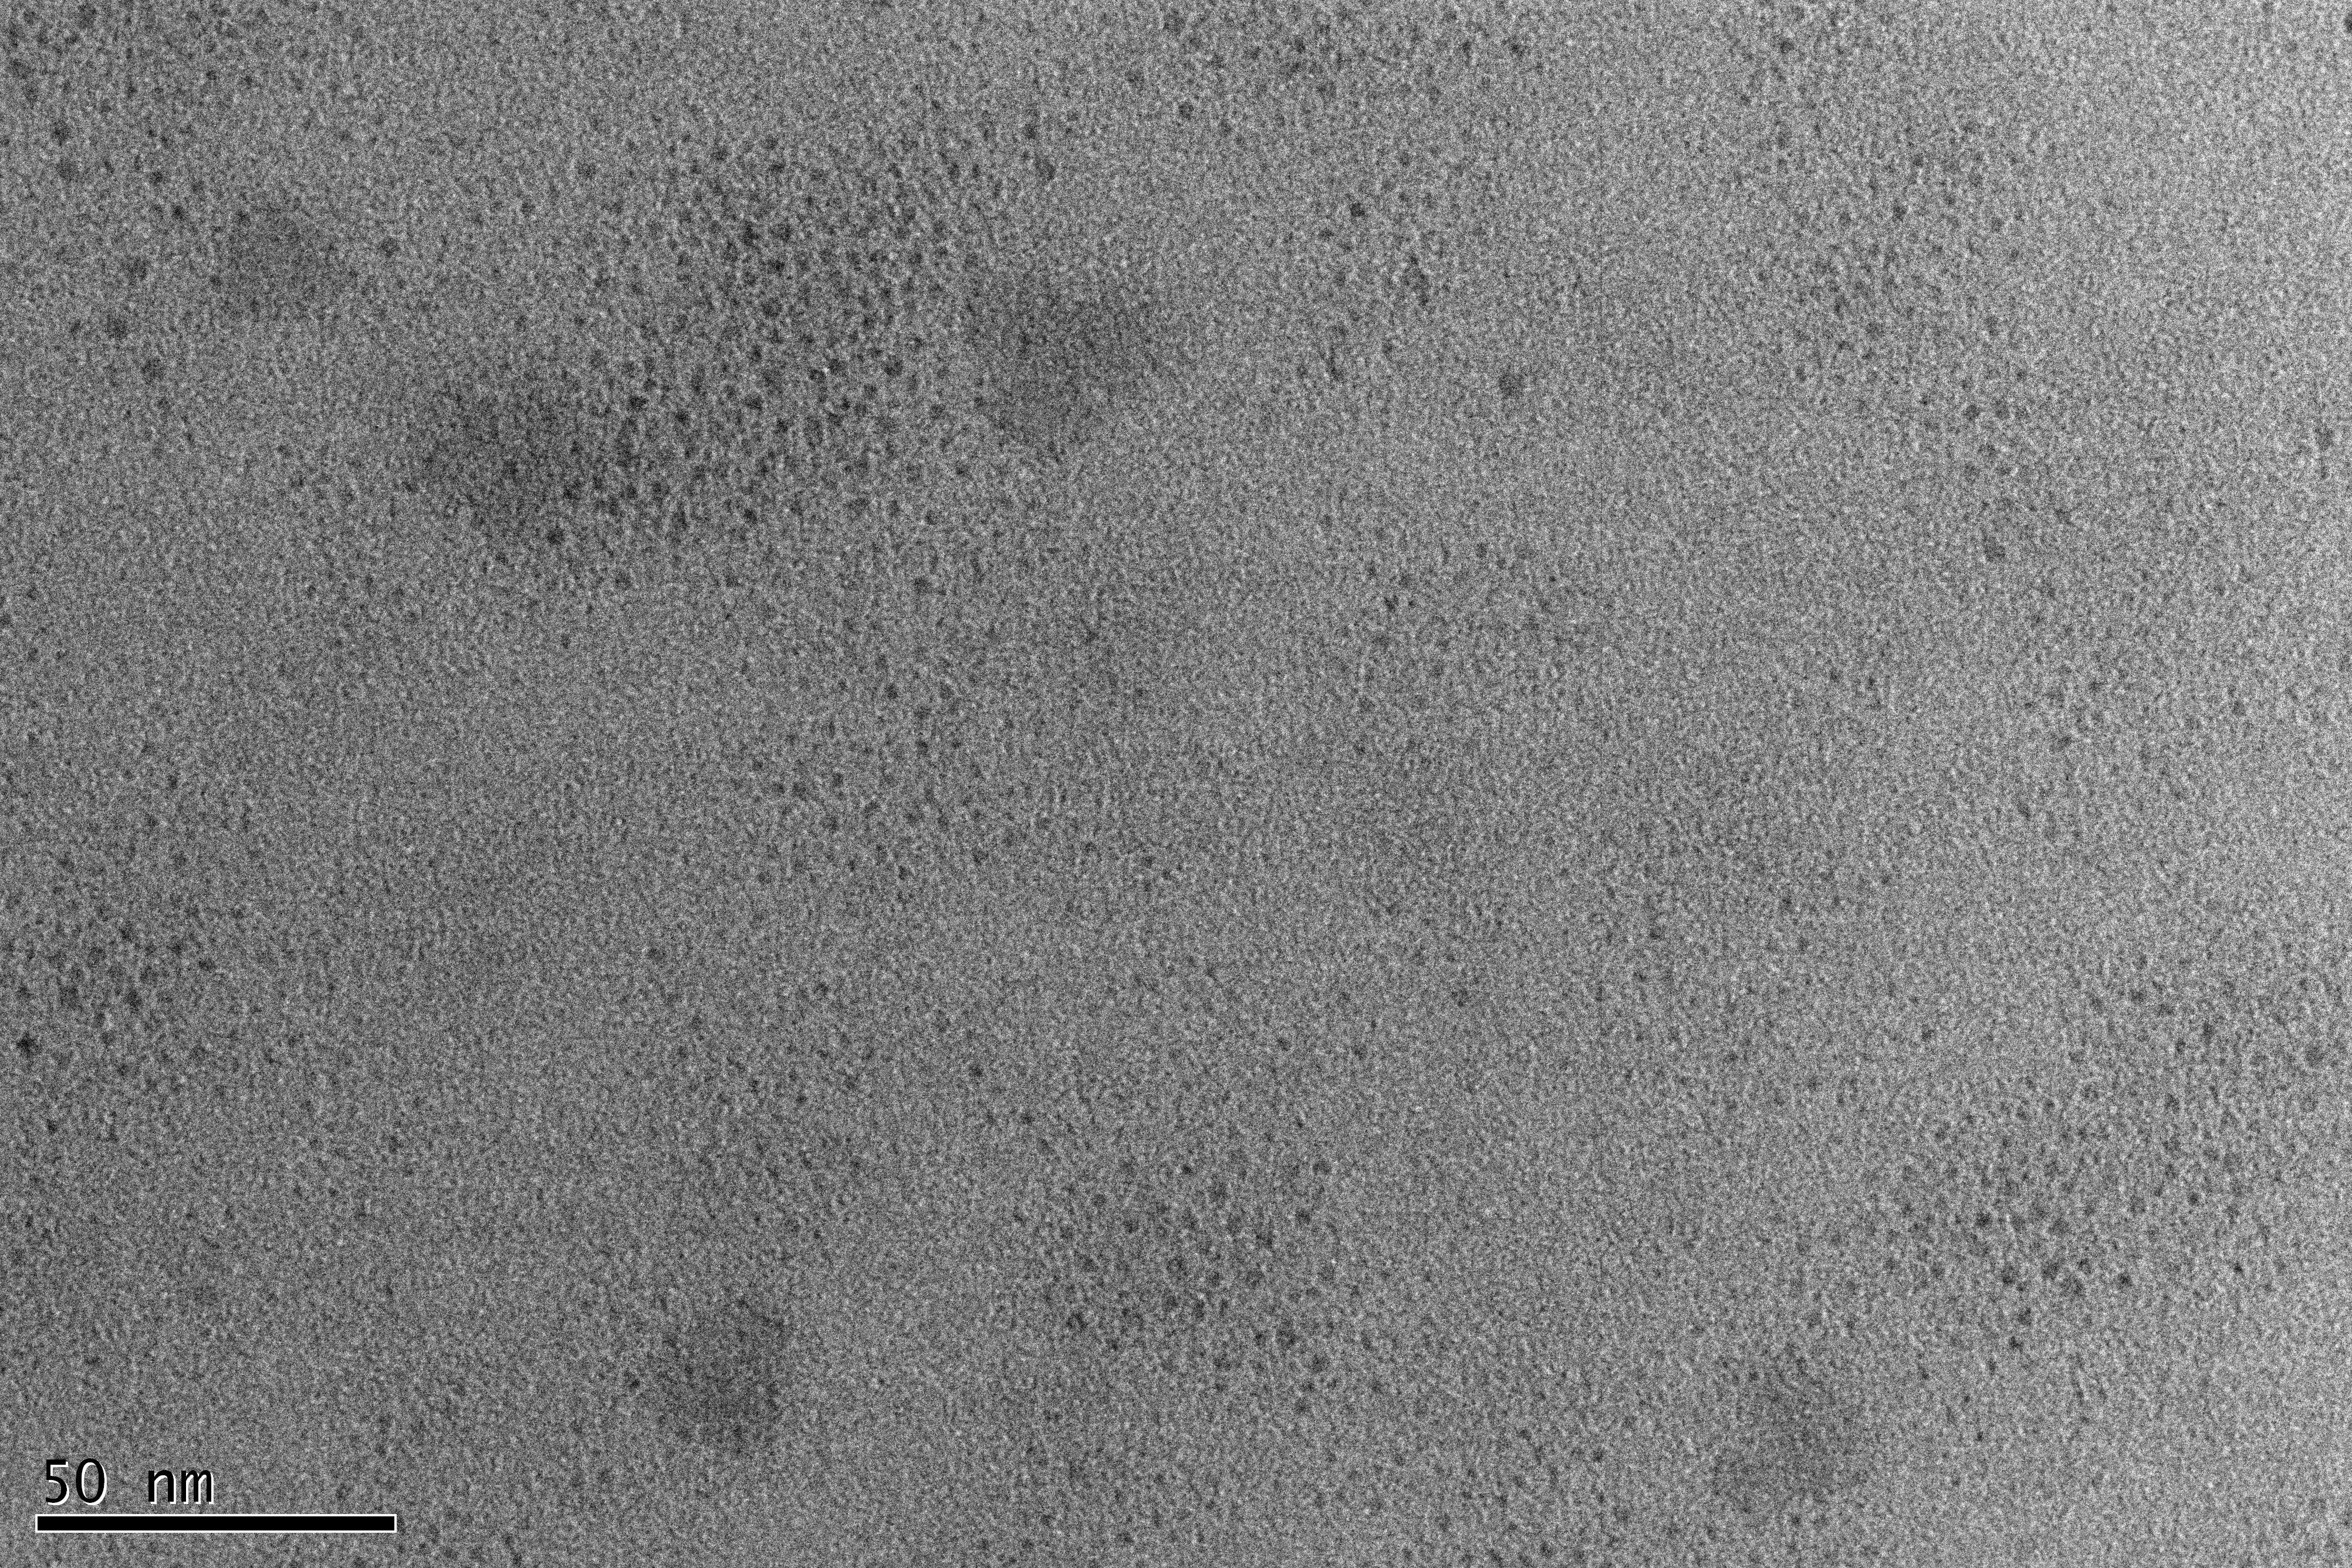
\includegraphics[width=0.45\linewidth]{Bilder/CuCl-2}}	
		\caption{TEM-Bilder von CuS-Nanopartikel, aus einem Gemisch von 80\% \ch{Cu[DDTC]2} und 20\% \ch{CuCl2}.}
		\label{fig:TEM-CuCl}
	\end{figure}
	
\subsection{Synthese von Kupfersulfid in Anwesenheit von Goldnanopartikeln}

	Um das Nukleationsverhalten bei der CuS-Synthese zu Untersuchen, wurde diese Reaktion in Anwesenheit von Goldnanopartikeln in verschiedenen Verhältnissen untersucht.
	Es wurden von diesen Mischungen jeweils UV-vis-NIR-Absorptionsmessungen vorgenommen und von ausgewählten Proben TEM-Aufnahmen und XRD-Messungen vorgenommen.
	
	\begin{figure}[htbp]
		\centering
		\includegraphics[width=0.6\textwidth]{Bilder/UV-AuCu-Konz} 	
		\caption{UV-vis-NIR-Messungen der Proben mit verschieden Mischungsverhältnissen von Au:\ch{Cu[DDTC]2} in Toluol (gemessen in Ulbrichtkugel).}
		\label{fig:UV-AuCu}
	\end{figure}
	
	Die Absorptionsmessungen in \cref{fig:UV-AuCu} zeigen, dass bei den Mischungen mit geringem Goldanteil ein Maximum bei etwa \SI{500}{\nano\meter} entsteht, dass mit steigendem Goldanteil abnimmt.
	Dies könnte das Plasmon der Goldpartikel sein.
	Interessanterweise ist das Maximum bei diesen Mischungen leicht blauverschoben und teilweise ausgeprägter als bei einer Vergleichsprobe, bei der die gleiche Reaktion ohne \ch{Cu[DDTC]2} und nur mit der Gold-NP-Lösung durchgeführt wurde.
	
	Die TEM-Aufnahmen zeigen, dass bei den Proben sowohl mit einem hohen als auch bei einem niedrigen Au:\ch{Cu[DDTC]2}-Verhältnis es zu einzelnen kleinen Gruppen von Gold-NPs kommt, an denen sich nicht gebildet hat (\cref{fig:CuAu-10-10_2} bzw. \cref{fig:CuAu-10-1_2}).
	Bei geringem Goldanteil scheint ein Teil des \ch{Cu[DDTC]2} wie bei der Probe ohne Gold zu reinem hexagonalem CuS zu reagieren, wie \cref{fig:CuAu-10-1_3} zeigt.
	Insgesamt lässt sich hier aber erkennen, dass die CuS-Partikel in Anwesenheit von den Gold-NP sich deutlich anders ausbilden und es an einigen Stellen so aussieht, als währen dort Goldpartikel eingelagert, was besonders in \cref{fig:CuAu-10-1_1} zu erkennen ist.
	
	\begin{figure}[htbp]
		\centering
		\subfloat[\label{fig:CuAu-10-10_1}]{%
			\includegraphics[width=0.33\linewidth]{Bilder/CuAu-10-10_1}}
		\subfloat[\label{fig:CuAu-10-10_2}]{%
			\includegraphics[width=0.33\linewidth]{Bilder/CuAu-10-10_2}}
		\subfloat[\label{fig:CuAu-10-10_3}]{%
			\includegraphics[width=0.33\linewidth]{Bilder/CuAu-10-10_3}}
		\caption{TEM-Aufnahmen der Probe mit einem Mengenverhältnis von 1:1 Au:\ch{Cu[DDTC]2}.}
		\label{fig:TEM-CuAu-10-10}
	\end{figure}
	
	\begin{figure}[htbp]
		\centering
		\subfloat[\label{fig:CuAu-10-1_1}]{%
			\includegraphics[width=0.33\linewidth]{Bilder/CuAu-10-1_1}}
		\subfloat[\label{fig:CuAu-10-1_2}]{%
			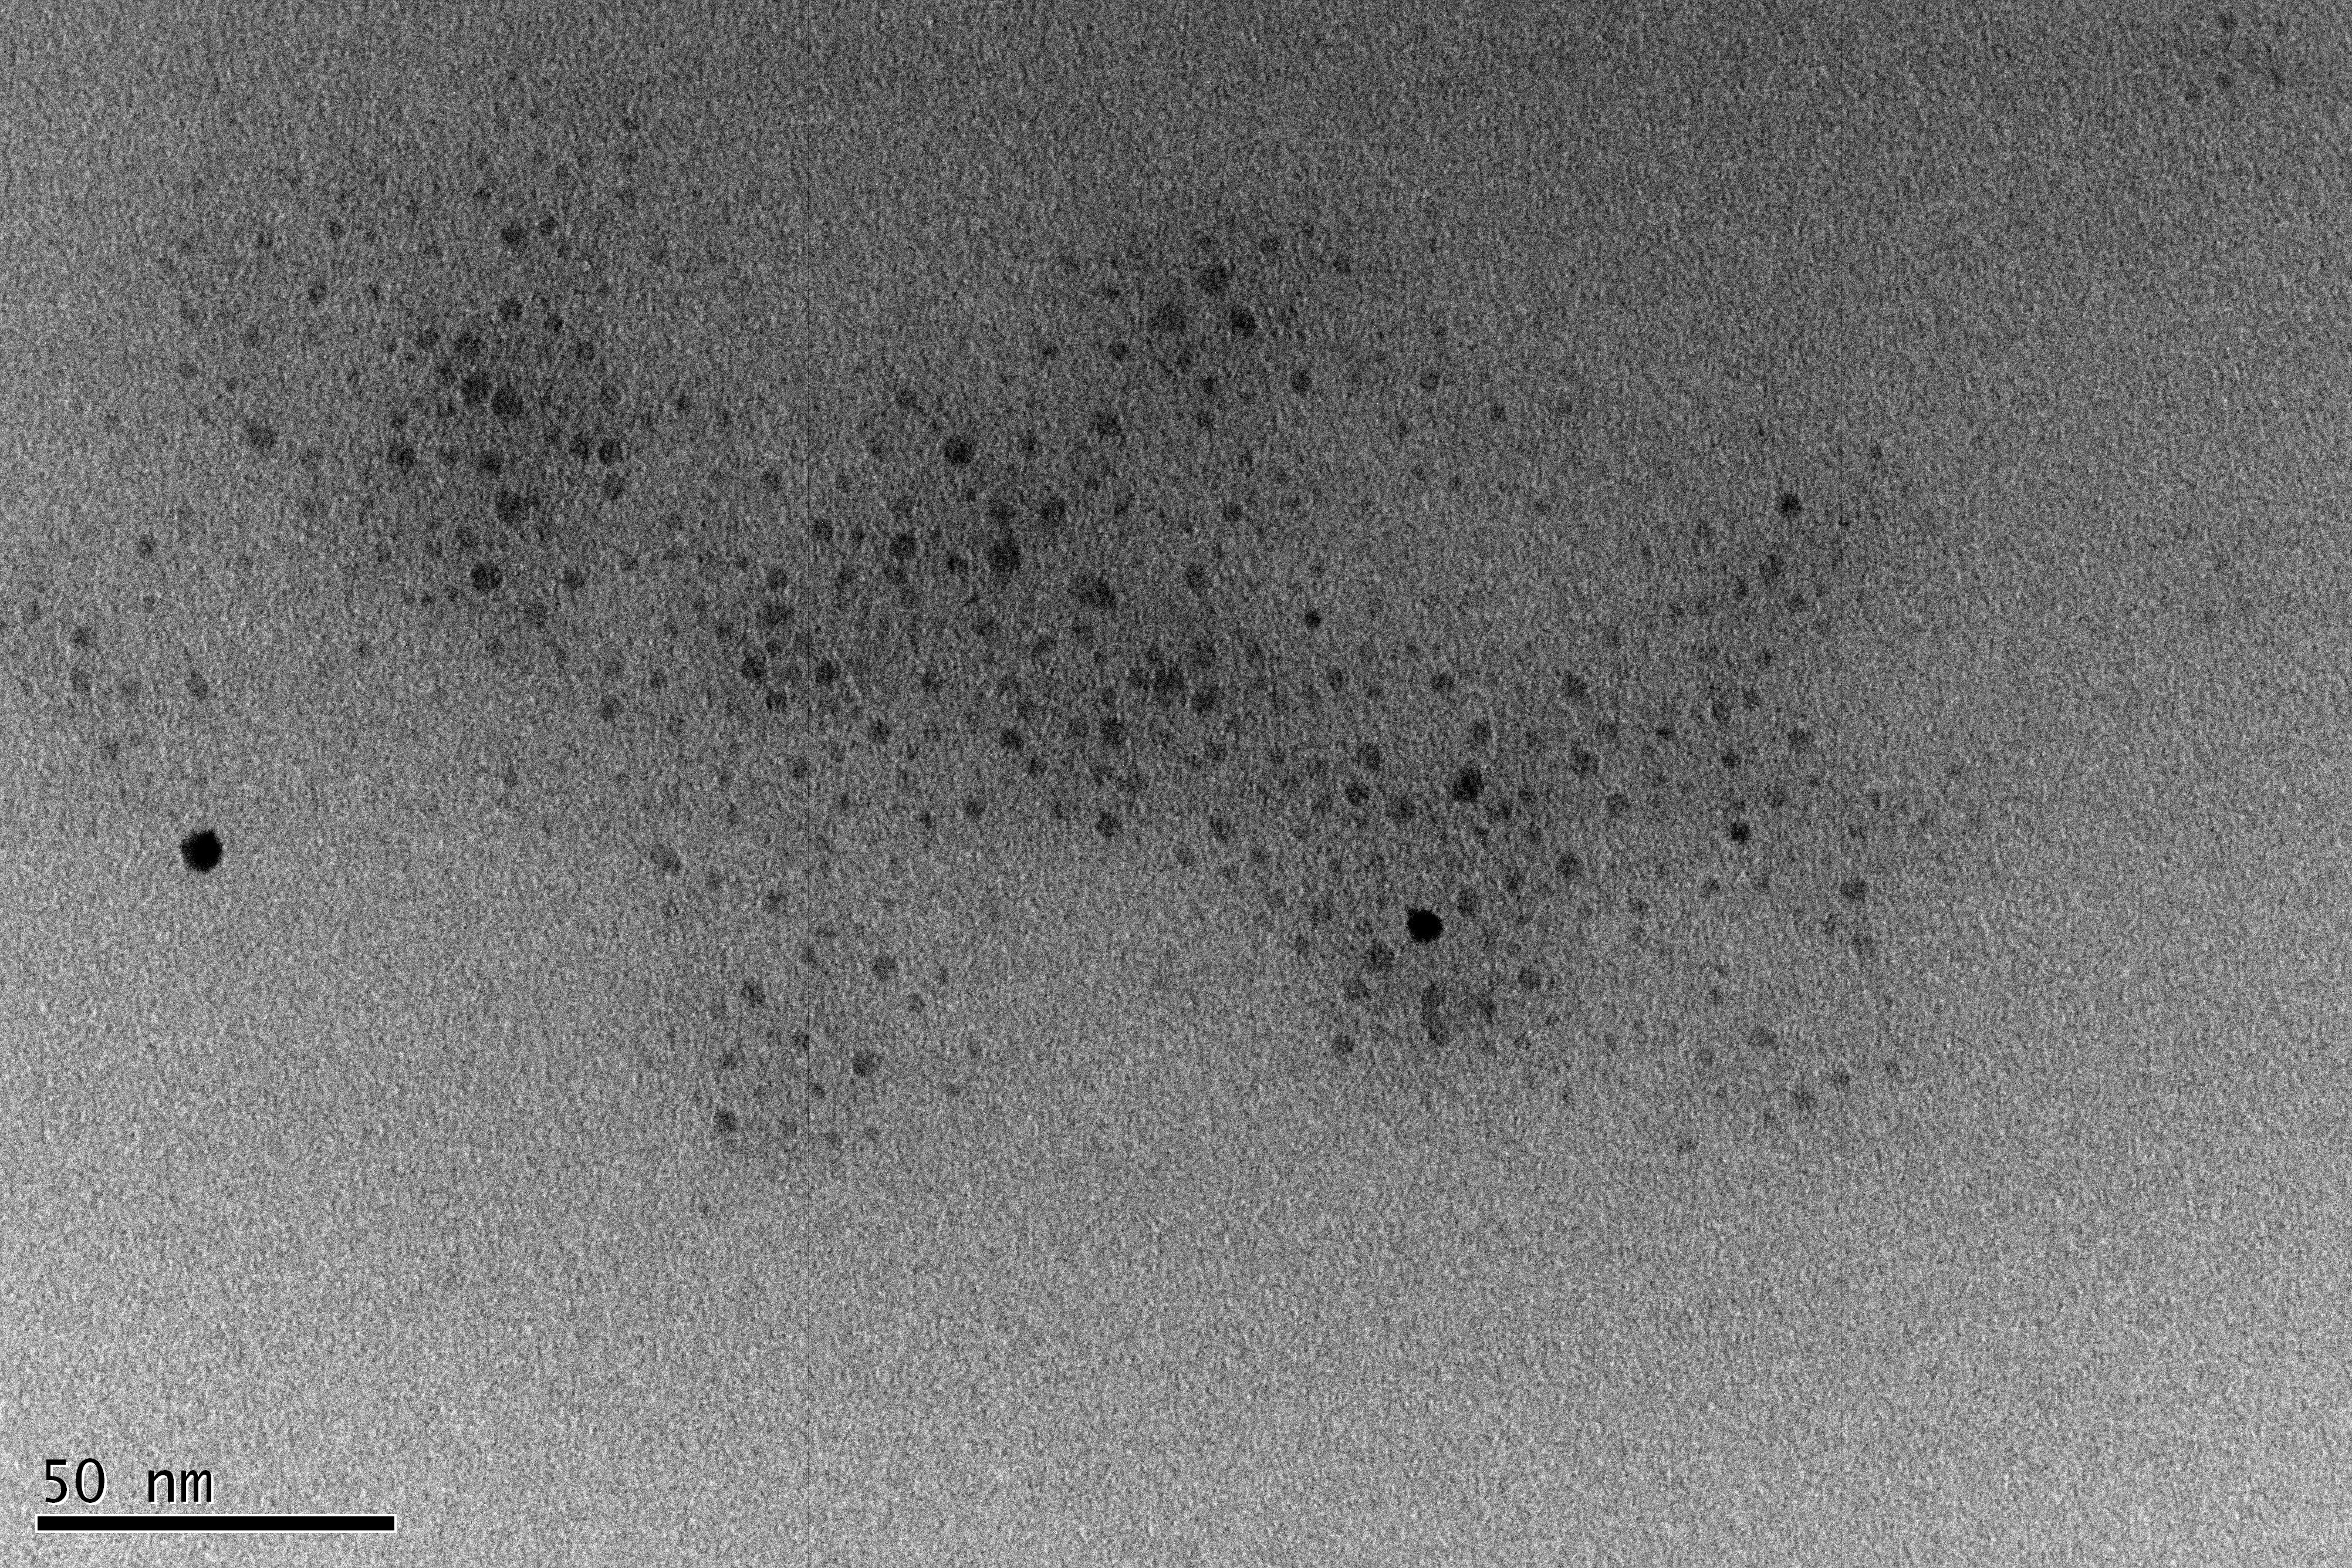
\includegraphics[width=0.33\linewidth]{Bilder/CuAu-10-1_2}}
		\subfloat[\label{fig:CuAu-10-1_3}]{%
			\includegraphics[width=0.33\linewidth]{Bilder/CuAu-10-1_3}}
		\caption{TEM-Aufnahmen der Probe mit einem Mengenverhältnis von 1:10 Au:\ch{Cu[DDTC]2}.}
		\label{fig:TEM-CuAu-10-1}
	\end{figure}
	
	Von den Mengenverhältnis 1:2 und 1:10 Au:\ch{Cu[DDTC]2} wurde zudem eine XRD-Messung vorgenommen, das in \cref{fig:XRD} gezeigt ist.
	Die 1:10-Probe ziegte einige scharfe Peaks zwischen 10° und 25°, die allerdings weder dem CuS, noch den Edukten zugeordnet werden können.
	Es konnte auch sonst keine Struktur gefunden werden, die hierfür in Frage kommt, die aus Kupfer und Schwefel besteht.
	Das XRD beim  Mengenverhältnis von 1:2 Au:\ch{Cu[DDTC]2} zeigt ein deutlich anderes Diffraktogramm, mit einem breiten Peak bei etwa 41° und zwei kleinen bei 46° und 48°. Auch diese passen zu keinem der Produkte oder Edukte.
	\todo{vielleicht Verschiebung des Gold-Peaks?}
	Es liegt der Verdacht nah, dass die Proben nicht kristallin genug waren um Signale im XRD zu erzeugen.
	
	\begin{figure}[H]
		\centering
		\includegraphics[width=\textwidth]{Bilder/XRD-CuS} 	
		\caption{XRD-Messung von Proben mit Mengenverhältnissen 1:2 und 1:10 Au:\ch{Cu[DDTC]2}.}
		\label{fig:XRD}
	\end{figure}
	
	
	
	

\subsection{Synthese der Gele}
	
	\subsubsection{Untersuchung von Hydrogelen durch Yttrium und Ytterbium}
	
		Bei fast allen Versuchen konnte nach einiger Zeit ein dunkler Niederschlag erkannt werden und die Lösung entfärbte sich bei fast allen Proben.
		Wie in \cref{fig:0625Au-Gele} zu erkennen ist, sind bei niedrigen Gold-NP-Konzentrationen von \SI{0,625}{\gram\per\liter} sowohl Yttrium als auch Ytterbium in allen verwendeten Konzentrationen in der Lage die in kolloidaler Lösung vorhandenen Goldnanopartikel auszufällen.
		Bei höheren Goldkonzentrationen konnte ein deutlicher Unterschied zwischen Ytterbium und Yttrium festgestellt werden. 
		Währenddessen die Yttriumlösungen auch die höheren Gold-NP-Konzentrationen von \num{1,25} und \SI{2,5}{\gram\per\liter} komplett ausfällen konnte, war dies mit Ytterbium in gleicher Konzentration nicht möglich, wie in \cref{fig:1Y-Yb-Gele} durch die immer noch vorhandene Rotfärbung zu erkennen ist.
		
		\begin{figure}[htbp]
			\centering
			\includegraphics[width=0.6\textwidth]{Bilder/0625Au-Gele} 	
			\caption{Übersicht der Gele mit 0,625 g/L Goldlösung und Salzlösungen mit 1;5;10 mM Yb$^{3+}$ und Y$^{3+}$.}
			\label{fig:0625Au-Gele}
		\end{figure}
	
		\begin{figure}[htbp]
			\centering
			\includegraphics[width=0.6\textwidth]{Bilder/1Y-Yb-Gele} 	
			\caption{Übersicht der Gele mit 10 mM Yb$^{3+}$ und Y$^{3+}$-Lösung und 2,5; 1,25; 0,625 g/L Gold-NP-Lösung.}
			\label{fig:1Y-Yb-Gele}
		\end{figure}
		
		Da es bei den Proben mit Yttrium immer zu einer vollständigen Entfärbung kam, also sämtliches Gold aus der Lösung abgelagert wurde, wurde sich bei weiteren Untersuchungen auf diese beschränkt.
		Um festzustellen, ob es sich bei dem gebildeten Niederschlag um Gele handelte wurden TEM-Aufnahmen von einigen Proben vorgenommen.
		Dabei wurden jeweils die Extreme der verwendeten Konzentrationen näher untersucht.
		
		\begin{figure}[htbp]
			\centering
			\subfloat[\label{fig:Au-Y-}]{%
				\includegraphics[width=0.45\linewidth]{Bilder/Au-Y-}}
			\subfloat[\label{fig:Au+Y-}]{%
				\includegraphics[width=0.45\linewidth]{Bilder/Au+Y-}}\\
			\subfloat[\label{fig:Au-Y+}]{%
				\includegraphics[width=0.45\linewidth]{Bilder/Au-Y+}}
			\subfloat[\label{fig:Au+Y+}]{%
				\includegraphics[width=0.45\linewidth]{Bilder/Au+Y+}}
			\caption{TEM-Bilder nach Zugabe von Yttriumchlorid mit den Konzentrationen: \emph{(a)}:~Au:~\SI{0,625}{\gram\per\liter}, Y: 1~mM;
			\emph{(b)}:~Au:~\SI{2,5}{\gram\per\liter}, Y: 1~mM
			\emph{(c)}:~Au:~\SI{0,625}{\gram\per\liter}, Y: 10~mM
			\emph{(d)}:~Au:~\SI{2,5}{\gram\per\liter}, Y: 10~mM} 
			\label{fig:Y-Gele}
		\end{figure}
		
		Die TEM-Bilder zeigen, dass es zu deutlichen Unterschieden bei den verschiedenen Konzentrationen kommt.
		So entstehen bei hoher Goldkonzentration und niedriger Yttriumkonzentration keine Gele sondern es entsteht einfach ein großer Klumpen (\cref{fig:Au+Y-}).
		Bei hoher Goldkonzentration und hoher Yttriumkonzentration hingegen liegen die Partikel alle seperat voneinander vor und es wurde also auch hier kein Gel gebildet(\cref{fig:Au+Y+}). 
		Bei den Versuchen mit den geringen Goldkonzentrationen konnte bei beiden Yttriumkonzentration eine Anlagerung der Gold-NP aneinander beobachtet werden.
		Bei geringer Yttriumkonzentration lagen jedoch ein größerer Teil der Partikel einzeln vor wie \cref{fig:Au-Y-} zeigt. 
		Das, was dem Aussehen klassischer Nanopartikelgele am nächsten kam war die Probe mit niedriger Goldkonzentration und höherer Yttriumkonzentration (\cref{fig:Au-Y+}). 
		Hier sind die Partikel miteinander venetzt und bildeten dabei Hohlräume.
		
		
		
	 
	
	
	\subsubsection{Untersuchung von citratstabilisierten Gelen}
		
		Die für die Gelierung hergestellten Silber- und Goldpartikeln wurden per UV-vis-Absorptionsspektroskopie untersucht.
		Sie zeigten typische Absorptionsmaxima bei $\lambda_{Gold}$=\SI{525}{\nano\meter} und $\lambda_{Silber}$=\SI{412}{\nano\meter}, wie \cref{fig:Abs-cit} zeigt.
		\begin{figure}[H]
			\centering
			\includegraphics[width=0.6\textwidth]{Bilder/Citrat-NP} 	
			\caption{UV-vis-Absorptionsspektren von Gold-NP und Silber-NP.}
			\label{fig:Abs-cit}
		\end{figure}
	
		Da bei den Versuchen mit reinem Gold und Silber keine festen Gele entstanden sind wurden diese auch nicht weiter untersucht.
		Im Vergleich zu den Hydrogelen, ist das Gel während des Austausches der flüssigen Phase zu TOP zu etwa ein Drittel des Ausgangsvolumen zusammengeschrumpft.
		Von den bimetallischen Gelen aus Gold- und Silbernanopartikeln wurden TEM-Bilder nach dem Phasentransfer in TOP aufgenommen.
		Es ist ein Netzwerk zu erkennen, dass aus kleinen Partikeln ($\approx$~\SI{10}{\nano\meter}), die miteinander Verknüpft sind und dabei viele große Zwischenräume besitzt, wie \cref{fig:Gel-C} zeigt. 
		
		\begin{figure}[htbp]
			\centering
			\subfloat[\label{fig:Gel-C-1}]{%
				\includegraphics[width=0.33\linewidth]{Bilder/Gel-C-1}}
			\subfloat[\label{fig:Gel-C-2}]{%
				\includegraphics[width=0.33\linewidth]{Bilder/Gel-C-2}}
			\subfloat[\label{fig:Gel-C-3}]{%
				\includegraphics[width=0.33\linewidth]{Bilder/gel-C-3}}
			\caption{TEM-Bilder der citratstrabilisierten Gele in TOP}
			\label{fig:Gel-C}
		\end{figure}
		
	\subsubsection{Untersuchung der Gele aus ethanolischem Ansatz}
		
		Da bei diesen Gelen der Schritt der Nukleation und der Schritt der Gelierung nicht separat voneinander Ablaufen, war ein groberes, weniger gleichmäßiges Gel als bei den citratstabilisierten zu erwarten.
		Dies war auch wie \cref{fig:Gel-C} zeigt der Fall.
		Insgesamt zeigt das Gel weniger Zwischenräume bei einem deutlich größeren Partikeldurchmesser ($\approx$~\SI{100}{\nano\meter}).
		
		\begin{figure}[htbp]
			\centering
			\subfloat[\label{fig:Gel-E-1}]{%
				\includegraphics[width=0.45\linewidth]{Bilder/Gel-E-1}}
			\subfloat[\label{fig:Gel-E-2}]{%
				\includegraphics[width=0.45\linewidth]{Bilder/Gel-E-2}}
			\caption{TEM Bilder der Gele aus ethanolischem Ansatz}
			\label{fig:Gel-E}
		\end{figure}
	
	\subsection{Untersuchung der Metallsulfidsynthese in Anwesenheit von Gelen}
	
	Nachdem die Proben mit Goldpartikeln zeigten, dass bei der thermischen Zersetzung von \ch{Cu[DDTC]2} sich CuS nicht nur getrennt vom Gold bildet, wurde hier getestet ob sich CuS (und später auch CdS und ZnS) an schon vorhandene Gele anlagert bzw. anwächst und mit welchen Parametern man dieses Verhalten beeinflussen kann.
	Dabei wurde hauptsächlich mit den Gelen aus ethanolischem Ansatz gearbeitet.
	
	Es zeigt sich direkt, dass wie zu erwarten die Gele zusammenschrumpfen, während des Verdampfungsprozesses.
	Allerdings sind diese Xerogele nicht so stark geschrumpft wie man es von anderen Gelen teilweise kennt, was mit der relativ groben Struktur der Gele und verhältnismäßig kleinen Zwischenräumen, die kollabieren können, zusammenhängt.
	
	\begin{figure}[htbp]
	\centering
	\subfloat[\label{fig:vorher}]{%
		\includegraphics[width=0.45\linewidth]{Bilder/Muster}}
	\subfloat[\label{fig:nachher}]{%
		\includegraphics[width=0.45\linewidth]{Bilder/Muster}}
	\caption{}
	\label{fig:vn}
	\end{figure} 

	Die TEM-Aufnahmen des Gels, das mit \ch{Cu[DDTC]2} bei \SI{290}{\degreeCelsius} bearbeitet wurde zeigt, dass sich CuS am Gel gebildet hat.
	Von einer kompletten Schale ist es noch weit entfernt, aber zeigt, dass es möglich ist, mittels  thermischer Zersetzung von \ch{Cu[DDTC]2} das daraus entstehende CuS daran anzulagern.
	
	\begin{figure}[htbp]
		\centering
		\subfloat[\label{fig:Gel-E-Cu_1}]{%
			\includegraphics[width=0.45\linewidth]{Bilder/Gel-E-Cu_1}}
		\subfloat[\label{fig:Gel-E-Cu_2}]{%
			\includegraphics[width=0.45\linewidth]{Bilder/Gel-E-Cu_2}}
		\caption{TEM von einem ethanolischen Au-Gel mit CuS}
		\label{fig:E-Cu}
	\end{figure}

	
	   
	
 
 